%%
%% Author: Moritz
%% 18.03.2018
%%

% Preamble
\documentclass[../../Pflichtenheft.tex]{subfiles}
\begin{document}
    \newpage
    \subsection{Reservierungsdetail}
    \begin{figure}[ht!]
        \begin{center}
            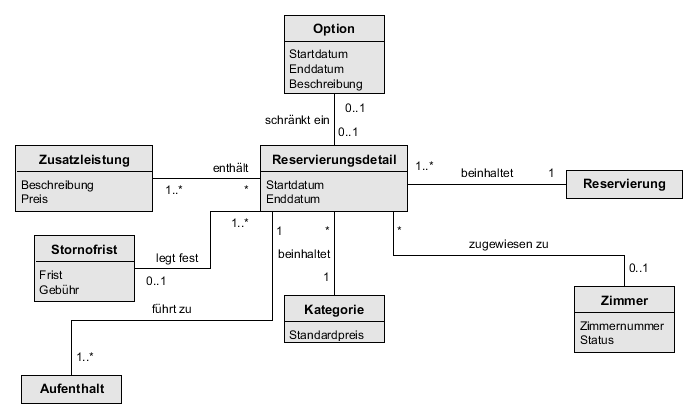
\includegraphics[width=0.5\linewidth]{assets/reservierungDetail.png}
            \caption{Objekt 'Reservierungsdetail'} \label{reservierungDetail_model}
        \end{center}
    \end{figure}
    Ein Reservierungsdetail enthält alle wichtigen Details und Informationen, welche für eine
    Reservierung notwendig sind. Zum Einen ist eine Option an ein Reservierungsdetail gebunden, die
    eine Frist für eine eventuelle Anzahlung festlegt. Zusatzleistungen sind ebenso an ein Reservierungsdetail
    geknüpft. Zudem werden Reservierungsdetails auf eine Kategorie gebucht oder auf expliziten Wunsch des
    Gastes, direkt mit einem Zimmer assoziiert. Die Stornofrist gibt die Stornierungsgebühren, sowie eine Frist,
    an, die festlegt, bis zu welchem Zeitpunkt man das Reservierungsdetail stornieren kann. Wenn der Gast
    eincheckt, werden Reservierungsdetails mit Aufenhalt, wobei aber alle Informationen aus dem Reservierungsdetail erhalten bleiben, verknüpft.
\end{document}